\chapter{Angular-Momentum Multiplets, Radial Motion, and the Oscillator Ladder}

\section{Angular Dependence of the Wavefunction}

A particle in a central force field has a radial position and two angular coordinates. Classically,
\begin{equation}
\mathbf L=\mathbf r\times\mathbf p
\end{equation}
is conserved as a vector. Its direction fixes the plane of the orbit, although the orbit need not be circular.

Quantum mechanically the particle is described by
\begin{equation}
\Psi=\Psi(r,\theta,\phi),
\end{equation}
and angular momentum concerns the dependence of this wavefunction on the angles.

In two dimensions there is only one angular-momentum component, the generator of rotations about the axis perpendicular to the plane:
\begin{equation}
L_z=-i\hbar\frac{\partial}{\partial\theta}.
\end{equation}
An eigenfunction with eigenvalue \(\hbar\ell\) obeys
\begin{equation}
-i\hbar\frac{\partial}{\partial\theta}\psi(r,\theta)
=\hbar\ell\,\psi(r,\theta).
\end{equation}
The coordinate \(r\) is a spectator in this equation. Its solution has the form
\begin{equation}
\psi(r,\theta)=\chi(r)e^{i\ell\theta}.
\end{equation}
For an ordinary single-valued orbital wavefunction, returning to the same point after \(\theta\to\theta+2\pi\) requires \(\ell\) to be an integer. The radial factor \(\chi(r)\) may affect the energy, but it does not affect this angular-momentum eigenvalue.

The three-dimensional analogue separates the radial dependence from functions on the sphere:
\begin{equation}
\Psi(r,\theta,\phi)=R(r)Y_{\ell m}(\theta,\phi).
\end{equation}
The functions \(Y_{\ell m}\) are spherical harmonics. Their explicit formulas will not be needed here. Rotations act on the angular factor, while the radial function is left alone.

\section{Finite Angular-Momentum Multiplets}

The components of angular momentum satisfy
\begin{equation}
[L_x,L_y]=i\hbar L_z,\qquad
[L_y,L_z]=i\hbar L_x,\qquad
[L_z,L_x]=i\hbar L_y.
\end{equation}
Choose eigenstates of \(L_z\),
\begin{equation}
L_z|\ell,m\rangle=\hbar m\,|\ell,m\rangle,
\end{equation}
and define
\begin{equation}
L_\pm=L_x\pm iL_y.
\end{equation}
The commutators
\begin{equation}
[L_z,L_\pm]=\pm\hbar L_\pm
\end{equation}
give
\begin{align}
L_z\bigl(L_\pm|\ell,m\rangle\bigr)
&=\bigl(L_\pm L_z+[L_z,L_\pm]\bigr)|\ell,m\rangle \\
&=\hbar(m\pm1)L_\pm|\ell,m\rangle.
\end{align}
Thus \(L_+\) raises \(m\) by one and \(L_-\) lowers it by one, unless the resulting vector vanishes.

For a finite multiplet there is a highest state and a lowest state:
\begin{equation}
L_+|\ell,\ell\rangle=0,
\qquad
L_-|\ell,-\ell\rangle=0.
\end{equation}
The \(+z\) and \(-z\) directions are related by a rotation, so the finite spectrum is symmetric about zero. Its values are therefore
\begin{equation}
m=-\ell,-\ell+1,\ldots,\ell-1,\ell,
\end{equation}
and the number of states is
\begin{equation}
2\ell+1.
\end{equation}
Since neighboring values differ by one, the endpoints can be integers or half-integers. Ordinary orbital spherical harmonics realize the integer case; the abstract angular-momentum algebra also permits half-integer multiplets.

\begin{classroomqa}
\lecturetimestamp{00:16:12}
\audiencequestion{Could an angular-momentum multiplet contain infinitely many states?}
\lecturerresponse{That possibility can be contemplated, but it will not be needed here. Angular momentum generally raises the energy when the other features of the state are held fixed, so states of infinite angular momentum are not relevant when discussing finite-energy states.}
\end{classroomqa}

\section{The Common Value of \(L^2\)}

The operator measuring the square of the angular-momentum magnitude is
\begin{equation}
L^2=L_x^2+L_y^2+L_z^2.
\end{equation}
The ordered product of ladder operators is
\begin{align}
L_-L_+
&=(L_x-iL_y)(L_x+iL_y) \\
&=L_x^2+L_y^2+i[L_x,L_y] \\
&=L_x^2+L_y^2-\hbar L_z.
\end{align}
Consequently,
\begin{equation}
L^2=L_z^2+\hbar L_z+L_-L_+.
\end{equation}
Apply this identity to the highest state. Since \(L_+|\ell,\ell\rangle=0\),
\begin{align}
L^2|\ell,\ell\rangle
&=\left(L_z^2+\hbar L_z+L_-L_+\right)|\ell,\ell\rangle \\
&=\hbar^2\left(\ell^2+\ell\right)|\ell,\ell\rangle,
\end{align}
and therefore
\begin{equation}
L^2|\ell,\ell\rangle
=\hbar^2\ell(\ell+1)|\ell,\ell\rangle.
\end{equation}
The squared magnitude is not \(\hbar^2\ell^2\). The extra term is a consequence of the noncommutativity of the angular-momentum components.

The same value belongs to every state in the multiplet, not only to the highest one.

\begin{classroomqa}
\lecturetimestamp{00:26:08}
\audiencequestion{What exactly is the exercise showing that the other states have the same value of \(L^2\)?}
\lecturerresponse{Show that \(L^2\) commutes with every component of angular momentum and hence with \(L_-\). Then commute \(L^2\) through \(L_-\): if the highest state has eigenvalue \(\hbar^2\ell(\ell+1)\), the next state down has the same eigenvalue. Repeating the argument carries that value through the whole ladder.}
\end{classroomqa}

Indeed,
\begin{equation}
[L^2,L_i]=0,
\qquad i=x,y,z,
\end{equation}
so
\begin{equation}
[L^2,L_\pm]=0.
\end{equation}
For example,
\begin{align}
L^2\bigl(L_-|\ell,\ell\rangle\bigr)
&=L_-L^2|\ell,\ell\rangle \\
&=\hbar^2\ell(\ell+1)L_-|\ell,\ell\rangle.
\end{align}
Continuing downward gives
\begin{equation}
L^2|\ell,m\rangle
=\hbar^2\ell(\ell+1)|\ell,m\rangle
\end{equation}
for every \(m=-\ell,\ldots,\ell\).

The opposite ordering gives an equivalent factorization:
\begin{align}
L_+L_-
&=(L_x+iL_y)(L_x-iL_y) \\
&=L_x^2+L_y^2-i[L_x,L_y] \\
&=L_x^2+L_y^2+\hbar L_z,
\end{align}
and hence
\begin{equation}
L^2=L_z^2-\hbar L_z+L_+L_-.
\end{equation}

\begin{classroomqa}
\lecturetimestamp{00:32:05}
\audiencequestion{Could \(L_x^2+L_y^2\) be factored in the opposite order using \(L_+L_-\)?}
\lecturerresponse{Yes. The sign of the \(L_z\) term reverses. With that ordering, apply the identity to the lowest state, which is annihilated by \(L_-\), rather than to the highest state. The same eigenvalue \(\hbar^2\ell(\ell+1)\) follows.}
\end{classroomqa}

The spherical harmonics therefore satisfy
\begin{align}
L^2Y_{\ell m}
&=\hbar^2\ell(\ell+1)Y_{\ell m}, \\
L_zY_{\ell m}
&=\hbar m\,Y_{\ell m}.
\end{align}
For each orbital value \(\ell=0,1,2,\ldots\), there are \(2\ell+1\) functions labeled by \(m=-\ell,\ldots,\ell\).

For a central potential,
\begin{equation}
[H,L_i]=0.
\end{equation}
Once a radial energy eigenstate and \(\ell\) are held fixed, changing \(m\) with \(L_\pm\) does not change the energy. Each such radial eigenstate therefore generates a \(2\ell+1\)-dimensional magnetic multiplet.

The integer orbital ladder is shown below.\footnote{The diagram is reconstructed from the multiplet sketch and operator identities visible at \(00{:}35{:}53\) of the lecture video.}

\begin{figure}[htbp]
\centering
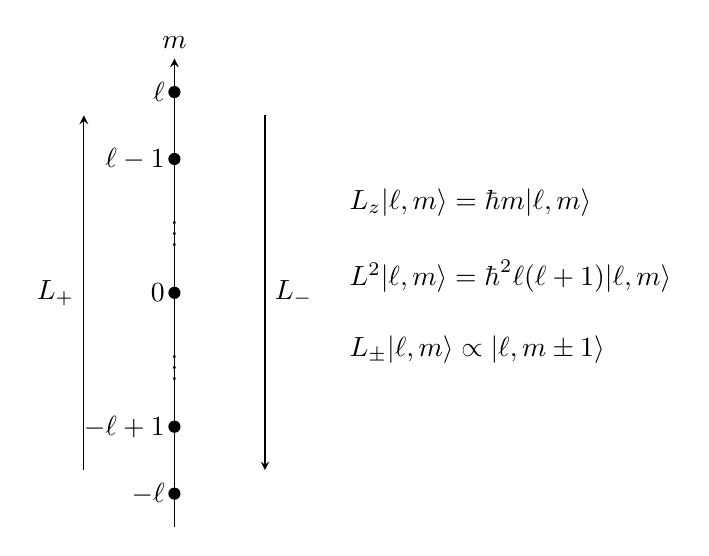
\begin{tikzpicture}[x=1cm,y=0.85cm,>=stealth]
\draw[->] (0,-3.5) -- (0,3.5) node[above] {$m$};

\fill (0,3) circle (2.2pt);
\fill (0,2) circle (2.2pt);
\fill (0,0) circle (2.2pt);
\fill (0,-2) circle (2.2pt);
\fill (0,-3) circle (2.2pt);

\node[left] at (0,3) {$\ell$};
\node[left] at (0,2) {$\ell-1$};
\node[left] at (0,0) {$0$};
\node[left] at (0,-2) {$-\ell+1$};
\node[left] at (0,-3) {$-\ell$};

\node at (0,1) {$\vdots$};
\node at (0,-1) {$\vdots$};

\draw[->] (-1.15,-2.65) -- (-1.15,2.65)
node[midway,left] {$L_+$};
\draw[->] (1.15,2.65) -- (1.15,-2.65)
node[midway,right] {$L_-$};

\node[anchor=west] at (2.1,1.35)
{$L_z|\ell,m\rangle=\hbar m|\ell,m\rangle$};
\node[anchor=west] at (2.1,0.25)
{$L^2|\ell,m\rangle=\hbar^2\ell(\ell+1)|\ell,m\rangle$};
\node[anchor=west] at (2.1,-0.85)
{$L_\pm|\ell,m\rangle\propto|\ell,m\pm1\rangle$};
\end{tikzpicture}
\caption{An integer orbital angular-momentum multiplet. \(L_+\) and \(L_-\) change \(m\) by one, while \(L^2\) remains \(\hbar^2\ell(\ell+1)\) throughout the multiplet.}
\lectureframe{00:35:53}
\end{figure}

\section{The Central-Force Problem}

Consider
\begin{equation}
H=\frac{\mathbf p^2}{2m}+V(r),
\end{equation}
where \(V\) depends only on the distance from the origin. Rotational symmetry implies conservation of angular momentum. Classically, \(\mathbf L\) has fixed magnitude and direction, so the orbit remains in a plane perpendicular to \(\mathbf L\). The orbit need not be circular, or even closed.

Choose coordinates so that this classical orbital plane is the \(xy\)-plane, and resolve the momentum into radial and tangential components:
\begin{equation}
\mathbf p^2=p_r^2+p_\theta^2.
\end{equation}
Since the magnitude of the angular momentum is
\begin{equation}
L=r p_\theta,
\end{equation}
the tangential contribution may be written
\begin{equation}
p_\theta^2=\frac{L^2}{r^2}.
\end{equation}
The Hamiltonian becomes
\begin{equation}
H=\frac{p_r^2}{2m}+\frac{L^2}{2mr^2}+V(r).
\end{equation}
For fixed \(L\), this is a one-dimensional problem in the radial coordinate, with effective potential
\begin{equation}
V_{\mathrm{eff}}(r)=\frac{L^2}{2mr^2}+V(r).
\end{equation}
The radial Hamiltonian is shown on the blackboard below.\footnote{Source frame: \texttt{\detokenize{lecture_03_frame_02.png}}, lecture video at \(00{:}47{:}15\).}

\begin{figure}[htbp]
\centering

\includegraphics[width=0.9\linewidth]{lecture_03_frame_02.png}
\caption{For fixed classical angular momentum, the radial Hamiltonian contains radial kinetic energy, the centrifugal term \(L^2/(2mr^2)\), and the central potential \(V(r)\).}
\lectureframe{00:47:15}
\end{figure}

The \(1/r^2\) term is the centrifugal barrier. It rises as the particle approaches the origin, so the associated force points outward. For the Coulomb-like attractions under discussion, a trajectory with \(L\neq0\) swings around the center instead of reaching it. When \(L=0\), the barrier is absent.

For the attractive Coulomb potential,
\begin{equation}
V(r)=-\frac{\kappa}{r},
\end{equation}
the centrifugal term dominates at small \(r\), while the Coulomb term falls more slowly and dominates at large \(r\). For \(L\neq0\), their sum has a minimum. Motion at the minimum has constant radius and is therefore circular. Bound motion above the minimum and below the escape threshold oscillates between a smallest and a largest radius; in the Coulomb problem these are the radial oscillations of an elliptical orbit.

\section{The Reduced Radial Equation}

In quantum mechanics the angular part of a state with definite orbital angular momentum is a spherical harmonic. Write the separated state as
\begin{equation}
\Psi_{n_r\ell m}(r,\theta,\phi)
=\frac{u_{n_r\ell}(r)}{r}\,
Y_{\ell m}(\theta,\phi).
\end{equation}
The angular operator \(L^2\) has the eigenvalue
\begin{equation}
L^2Y_{\ell m}
=\hbar^2\ell(\ell+1)Y_{\ell m}.
\end{equation}
The equation left for the reduced radial function is
\begin{equation}
\left[
-\frac{\hbar^2}{2m}\frac{d^2}{dr^2}
+\frac{\hbar^2\ell(\ell+1)}{2mr^2}
+V(r)
\right]u_{n_r\ell}(r)
=E_{n_r\ell}\,u_{n_r\ell}(r).
\end{equation}

\editorialnote{The pure one-dimensional second-derivative equation uses the reduced radial function \(u=rR\). Thus the \(\psi(r)\) in the displayed lecture equation corresponds to \(u(r)\), while the ordinary radial factor in \(\Psi=R(r)Y_{\ell m}\) is \(R=u/r\). This convention avoids treating \(-i\hbar\,d/dr\) as a standalone Hermitian radial-momentum operator on the three-dimensional radial Hilbert space.}

The reduced radial equation is shown on the blackboard below.\footnote{Source frame: \texttt{\detokenize{lecture_03_frame_03.png}}, lecture video at \(00{:}54{:}32\).}

\begin{figure}[htbp]
\centering

\includegraphics[width=0.9\linewidth]{lecture_03_frame_03.png}
\caption{For fixed \(\ell\), the reduced radial wavefunction satisfies a one-dimensional Schr\"odinger equation with a centrifugal term proportional to \(\ell(\ell+1)/r^2\).}
\lectureframe{00:54:32}
\end{figure}

The three-dimensional angular structure has been compressed into the parameter \(\ell\). The magnetic quantum number \(m\) does not occur in the radial equation.

\begin{classroomqa}
\lecturetimestamp{00:55:34}
\audiencequestion{For a given \(\ell\), do the \(2\ell+1\) magnetic states have the same energy?}
\lecturerresponse{Yes, provided the radial eigenstate is also held fixed. For each chosen \(u_{n_r\ell}\), all values \(m=-\ell,\ldots,\ell\) have the same energy because \(m\) does not enter the radial equation. Different radial eigenstates at the same \(\ell\) generally have different energies.}
\end{classroomqa}

\begin{classroomqa}
\lecturetimestamp{00:56:03}
\audiencequestion{Why may \(L^2\) be replaced by \(\hbar^2\ell(\ell+1)\), and how is \(\ell\) related to the allowed values of \(m\)?}
\lecturerresponse{The number \(\ell\) labels an angular-momentum multiplet and is its largest \(m\)-value. Every state in that multiplet has the same \(L^2\)-eigenvalue, \(\hbar^2\ell(\ell+1)\), so that eigenvalue is inserted into the radial equation.}
\end{classroomqa}

The explicit special-function solutions are not needed for the present argument. What matters is how the solutions are organized.

\section{Radial Nodes and Energy Levels}

For fixed \(\ell\), the reduced radial equation is an ordinary one-dimensional eigenvalue problem. Its bound states are ordered by their number of interior nodes. The lowest radial state has no interior node, the next has one, and the next has two. More nodes mean more rapid variation of the wavefunction; more rapid variation means larger momentum and therefore larger kinetic energy.

Each value of \(\ell\) defines a different radial operator because the centrifugal term changes with \(\ell\). Thus \(\ell=0,1,2,\ldots\) give separate radial towers. The positive centrifugal term shifts the levels upward as angular momentum is added. Every radial eigenvalue at fixed \(\ell\) carries a magnetic multiplet of dimension
\begin{equation}
2\ell+1.
\end{equation}
The \(\ell=0\) levels are singlets, the \(\ell=1\) levels are triplets, and the \(\ell=2\) levels are quintuplets. These are the degeneracies guaranteed by rotational symmetry; an additional symmetry may make states with different values of \(\ell\) degenerate as well.

For atomic-type potentials satisfying \(V(r)\to0\) at large \(r\), the escape threshold is conventionally \(E=0\). The negative-energy states form the discrete bound spectrum. At and above \(E=0\), one encounters the scattering continuum. This statement depends on the large-\(r\) behavior of the potential and does not apply to a confining central potential.

\section{The Special Coulomb Degeneracy}

The exact nonrelativistic Coulomb potential has an additional alignment of levels. The lowest \(\ell=1\) radial state has the same energy as the first excited \(\ell=0\) state. The next \(\ell=1\) state aligns with the second excited \(\ell=0\) state, and the lowest \(\ell=2\) state joins them. The pattern continues through the higher radial and angular-momentum towers.

\begin{classroomqa}
\lecturetimestamp{01:09:57}
\audiencequestion{Does this extra Coulomb degeneracy indicate another symmetry?}
\lecturerresponse{Yes. It is an unusual additional symmetry of the exact Coulomb potential. Small changes in the potential destroy the alignment, and its derivation is not pursued here.}
\end{classroomqa}

The resulting orbital shell degeneracies are
\begin{equation}
1,\qquad 4,\qquad 9,\qquad 16,\qquad \ldots
\end{equation}
before electron spin is included.

\begin{classroomqa}
\lecturetimestamp{01:11:46}
\audiencequestion{Does this degeneracy describe hydrogen, or only the ideal Coulomb problem?}
\lecturerresponse{Hydrogen satisfies it to very good approximation, but not exactly. Relativistic corrections and the finite size of the nucleus disturb the ideal Coulomb pattern.}
\end{classroomqa}

A point nucleus produces an exact \(1/r\) potential. A nucleus with charge spread over a small volume produces a slightly different potential when the electron penetrates that volume, and even this small departure lifts part of the special degeneracy.

Spin has also been omitted. Including the two electron spin states doubles the shell counts to
\begin{equation}
2,\qquad 8,\qquad 18,\qquad 32,\qquad \ldots
\end{equation}
before the further splittings of a more complete atomic treatment are resolved.

\section{The Cartesian Equation Revisited}

The equation from which the radial problem began is the three-dimensional time-independent Schr\"odinger equation
\begin{equation}
-\frac{\hbar^2}{2m}
\left(
\frac{\partial^2}{\partial x^2}
+\frac{\partial^2}{\partial y^2}
+\frac{\partial^2}{\partial z^2}
\right)\Psi
+V\!\left(\sqrt{x^2+y^2+z^2}\right)\Psi
=E\Psi.
\end{equation}
Passing to radial and angular coordinates, selecting an \(L^2\)-eigenstate, and replacing \(L^2\) by \(\hbar^2\ell(\ell+1)\) reduces this partial differential equation to the ordinary radial equation above.

\begin{classroomqa}
\lecturetimestamp{01:16:42}
\audiencequestion{Could deviations from the ideal Coulomb spectrum be used to determine the size of the nucleus?}
\lecturerresponse{Not by this simple comparison. Other corrections are much larger and must first be accounted for. Nuclear size is mentioned here because it gives an immediate example of a departure from the point-Coulomb potential.}
\end{classroomqa}

\begin{classroomqa}
\lecturetimestamp{01:17:09}
\audiencequestion{What is the main difference between the classical and quantum angular-momentum terms?}
\lecturerresponse{Classically \(L^2\) is the ordinary square of a conserved vector magnitude. In a quantum orbital multiplet its eigenvalue is \(\hbar^2\ell(\ell+1)\), not simply \(\hbar^2\ell^2\). The additional term comes from the noncommutativity of the angular-momentum components.}
\end{classroomqa}

\begin{classroomqa}
\lecturetimestamp{01:17:58}
\audiencequestion{Do the bound-state wavefunctions have compact support?}
\lecturerresponse{No. They extend arbitrarily far from the center. For the atomic bound states under discussion they decrease exponentially at large distance, so the probability becomes negligible but does not vanish beyond any finite radius.}
\end{classroomqa}

\begin{classroomqa}
\lecturetimestamp{01:18:48}
\audiencequestion{When \(\ell=0\) removes the centrifugal well, what becomes of the stable point?}
\lecturerresponse{There is no longer a minimum produced by competition between the centrifugal barrier and the attraction. In the point-Coulomb idealization the classical motion heads toward the singular center. Quantum mechanically the lowest state cannot have both an exactly definite position at the center and zero momentum, so the lowest wavefunction has a finite spatial spread.}
\end{classroomqa}

\editorialnote{For a regular central potential, a classical zero-angular-momentum trajectory may continue through the origin. For the ideal point-Coulomb potential, \(r=0\) is instead a collision singularity, and continuation of the classical trajectory requires an additional prescription.}

The classical reduction placed a single orbit in a plane, but that step cannot be applied to a quantum wavefunction in the same way. A quantum orbital state fills three-dimensional space. The full angular operator is \(L^2=L_x^2+L_y^2+L_z^2\), and its eigenvalue retains the three-dimensional result \(\hbar^2\ell(\ell+1)\).

\begin{classroomqa}
\lecturetimestamp{01:21:30}
\audiencequestion{How can the quantum problem remain three-dimensional after the classical orbit was placed in a plane?}
\lecturerresponse{Only the classical orbit was put in a fixed plane by choosing coordinates perpendicular to its conserved angular-momentum vector. A quantum wavefunction occupies three-dimensional space. The other angular-momentum components remain present through \(L^2\), which is why the radial equation contains \(\ell(\ell+1)\) rather than only a square of one component.}
\end{classroomqa}

\begin{classroomqa}
\lecturetimestamp{01:22:54}
\audiencequestion{Does every quantum problem admit raising and lowering operators?}
\lecturerresponse{No. They occur in unusually favorable cases. Angular momentum is one such case, and the harmonic oscillator is another. The oscillator case is especially useful because motion near a stable equilibrium is so often approximately harmonic, including small radial oscillations near the minimum of an effective potential.}
\end{classroomqa}

The atomic problem is set aside at this point, and the harmonic oscillator becomes the next example of a spectrum determined by ladder operators.

\section{Small Oscillations and the Harmonic Oscillator}

Near a stable equilibrium, a sufficiently small displacement often produces harmonic motion. The effective radial potential for nonzero angular momentum provides one example: radial motion close to the bottom of its well is approximately harmonic.

Consider a one-dimensional oscillator with unit mass. Let \(x\) be the displacement from equilibrium and write the spring constant as \(k=\omega^2\). The classical Hamiltonian is
\begin{equation}
H=\frac{p^2}{2}+\frac{\omega^2x^2}{2}.
\end{equation}
Hamilton's equations give
\begin{equation}
\dot{x}=\frac{\partial H}{\partial p}=p,
\qquad
\dot{p}=-\frac{\partial H}{\partial x}=-\omega^2x,
\end{equation}
and therefore
\begin{equation}
\ddot{x}=-\omega^2x.
\end{equation}
Thus \(\omega\) is the classical oscillation frequency.

\section{Factorization and the Zero-Point Energy}

Quantum mechanically,
\begin{equation}
[x,p]=i\hbar.
\end{equation}
The Hamiltonian is a sum of squares, suggesting the factorization
\begin{align}
\frac{1}{2}(p+i\omega x)(p-i\omega x)
&=\frac{1}{2}\left(p^2+\omega^2x^2+i\omega[x,p]\right) \\
&=\frac{1}{2}\left(p^2+\omega^2x^2-\hbar\omega\right).
\end{align}
Hence
\begin{equation}
H=\frac{1}{2}(p+i\omega x)(p-i\omega x)
+\frac{1}{2}\hbar\omega.
\end{equation}
The additive term \(\hbar\omega/2\) is the zero-point energy.

Classically the lowest energy would occur at \(x=p=0\). Quantum mechanically no state can have both position and momentum sharply fixed at zero. Moreover, the two terms \(p^2/2\) and \(\omega^2x^2/2\) are positive and cannot cancel. A nonzero ground-state energy is therefore unavoidable.

For the ladder calculation the common additive constant may be set aside temporarily and restored at the end.

\begin{classroomqa}
\lecturetimestamp{01:36:10}
\audiencequestion{Does the positive sign of the zero-point term tell us anything further?}
\lecturerresponse{The oscillator Hamiltonian is a positive operator: it is a sum of positive squares, so its energy cannot be negative.}
\end{classroomqa}

\section{The Oscillator Ladder}

Introduce the dimensionless operators\footnote{Around \(01{:}37\)--\(01{:}42\), the calculation uses \(\hbar=1\). The factor of \(\hbar\) is restored in these normalized definitions so that \(A_\pm\) are dimensionless and their commutator is unity.}
\begin{equation}
A_+=\frac{p+i\omega x}{\sqrt{2\hbar\omega}},
\qquad
A_-=\frac{p-i\omega x}{\sqrt{2\hbar\omega}}.
\end{equation}
They are Hermitian conjugates:
\begin{equation}
A_+^\dagger=A_-.
\end{equation}
Their commutator is
\begin{align}
[A_-,A_+]
&=\frac{1}{2\hbar\omega}
\left([p,i\omega x]+[-i\omega x,p]\right) \\
&=1.
\end{align}

Define
\begin{equation}
N=A_+A_-.
\end{equation}
The Hamiltonian is then
\begin{equation}
H=\hbar\omega\left(N+\frac{1}{2}\right).
\end{equation}
Thus finding the energy spectrum reduces to finding the eigenvalues of \(N\).

Suppose
\begin{equation}
N|n\rangle=n|n\rangle.
\end{equation}
The commutators with \(N\) are\footnote{The intermediate steps at \(01{:}45{:}37\)--\(01{:}48{:}10\) are reconstructed directly from the stated relations \(N=A_+A_-\) and \([A_-,A_+]=1\).}
\begin{align}
[N,A_+]
&=A_+[A_-,A_+]=A_+, \\
[N,A_-]
&=[A_+,A_-]A_-=-A_-.
\end{align}
It follows that
\begin{align}
N\bigl(A_+|n\rangle\bigr)
&=(n+1)A_+|n\rangle, \\
N\bigl(A_-|n\rangle\bigr)
&=(n-1)A_-|n\rangle.
\end{align}
Thus \(A_+\) raises an eigenvalue of \(N\) by one and \(A_-\) lowers it by one whenever the resulting vector is nonzero.

The operator \(N\) is nonnegative:
\begin{equation}
\langle\psi|N|\psi\rangle
=\langle\psi|A_+A_-|\psi\rangle
=\|A_-|\psi\rangle\|^2
\geq0.
\end{equation}
The lowering process therefore cannot continue into negative eigenvalues. At a bottom state \(|b\rangle\), it must terminate:
\begin{equation}
A_-|b\rangle=0.
\end{equation}

For normalized eigenstates, the coefficients in the ladder are fixed by their norms:
\begin{align}
\|A_-|n\rangle\|^2
&=\langle n|A_+A_-|n\rangle=n, \\
\|A_+|n\rangle\|^2
&=\langle n|A_-A_+|n\rangle=n+1.
\end{align}
Phases may therefore be chosen so that
\begin{equation}
A_-|n\rangle=\sqrt{n}\,|n-1\rangle,
\qquad
A_+|n\rangle=\sqrt{n+1}\,|n+1\rangle.
\end{equation}

\begin{classroomqa}
\lecturetimestamp{01:52:42}
\audiencequestion{If \(A_-\) lowers a state and \(A_+\) raises it back, how does \(A_+A_-\) produce the eigenvalue \(n\)?}
\lecturerresponse{The ladder action includes normalization factors. Acting first with \(A_-\) contributes \(\sqrt n\), and acting with \(A_+\) on the resulting state contributes another \(\sqrt n\). Their product is \(n\).}
\end{classroomqa}

Indeed,
\begin{equation}
A_+A_-|n\rangle
=\sqrt n\,A_+|n-1\rangle
=n|n\rangle.
\end{equation}

\begin{classroomqa}
\lecturetimestamp{01:55:52}
\audiencequestion{Must the lowest eigenvalue of \(N\) be zero, or could it be positive?}
\lecturerresponse{It must be zero, and the spectrum of \(N\) consists of the nonnegative integers. A proof of the endpoint has not yet been supplied.}
\end{classroomqa}

\editorialnote{Let \(|b\rangle\) be a lowest state. Since lowering must terminate, \(A_-|b\rangle=0\). It follows immediately that \(N|b\rangle=A_+A_-|b\rangle=0\), so the lowest eigenvalue of \(N\) is zero.}

Starting from this lowest state and applying \(A_+\) gives
\begin{equation}
n=0,1,2,\ldots.
\end{equation}
Restoring the additive zero-point term, the oscillator energies are
\begin{equation}
E_n=\hbar\omega\left(n+\frac{1}{2}\right),
\qquad n=0,1,2,\ldots.
\end{equation}

The oscillator algebra will be developed further and used to solve other quantum problems.
